\documentclass[10pt,aspectratio=43]{beamer}

\usetheme{Darmstadt}
\useoutertheme{infolines}
\setbeamertemplate{navigation symbols}{}

% --- colours in the spirit of the CLASS bootcamp slides ----------------------
\definecolor{cgold}{RGB}{243,169,20}
\definecolor{cdeep}{RGB}{176,110,10}
\definecolor{cink}{RGB}{40,40,45}
\definecolor{cred}{RGB}{190,40,40}
\definecolor{cblue}{RGB}{30,80,160}

\setbeamercolor{structure}{fg=cdeep}
\setbeamercolor{palette primary}{bg=cgold,fg=cink}
\setbeamercolor{palette secondary}{bg=cdeep,fg=white}
\setbeamercolor{palette tertiary}{bg=cgold,fg=cink}
\setbeamercolor{frametitle}{bg=cgold,fg=cink}
\setbeamercolor{title}{bg=cgold,fg=cink}
\setbeamercolor{subtitle}{fg=cink}
\setbeamercolor{author}{fg=cink}
\setbeamercolor{block title}{bg=cgold,fg=cink}
\setbeamercolor{block body}{bg=cgold!12,fg=cink}
\setbeamercolor{alerted text}{fg=cred}
\setbeamerfont{frametitle}{series=\bfseries}
\setbeamertemplate{blocks}[rounded][shadow=true]
\setbeamertemplate{itemize item}{\color{cdeep}$\blacktriangleright$}
\setbeamertemplate{itemize subitem}{\color{cdeep}$\bullet$}

\usepackage[utf8]{inputenc}
\usepackage{amsmath,amssymb}
\usepackage{booktabs}
\usepackage{listings}
\usepackage{graphicx}
\usepackage{xcolor}

\lstdefinestyle{jl}{
  language=Java,
  basicstyle=\ttfamily\scriptsize,
  keywordstyle=\color{cblue}\bfseries,
  commentstyle=\color{gray}\itshape,
  stringstyle=\color{cdeep},
  showstringspaces=false,
  columns=fullflexible,
  morekeywords={using,function,end,for,in,struct,const,let,if,else,return,true,false},
  breaklines=true,
  frame=none,
  aboveskip=2pt, belowskip=2pt,
}
\lstset{style=jl}

\newcommand{\cl}{C_\ell}
\newcommand{\Cosmic}{\textcolor{cdeep}{\texttt{Cosmic.jl}}}

\title[Cosmic.jl]{\texttt{Cosmic.jl}}
\subtitle{A cosmology and Einstein--Boltzmann engine in pure Julia}
\author{Kazi Abu Rousan}
\date{\today}

\begin{document}

{\setbeamertemplate{headline}{}
\begin{frame}[plain]
  \titlepage
  \begin{center}
    \small\textcolor{cdeep}{\texttt{github.com/aburousan/Cosmic.jl}}
  \end{center}
\end{frame}}

\begin{frame}{Outline}
  \tableofcontents
\end{frame}

% =============================================================================
\section{Why}

\begin{frame}{Where this sits}
  Public Boltzmann codes, in order of appearance:
  \begin{enumerate}
    \item \textcolor{cdeep}{COSMICS} (f77, Bertschinger 1995) --- brute-force $\cl^{TT}$.
    \item \textcolor{cdeep}{CMBFAST} (Seljak \& Zaldarriaga 1996) --- the line-of-sight trick.
    \item \textcolor{cdeep}{CAMB} (Lewis, Challinor \& Lasenby 2000) --- Fortran; the workhorse.
    \item \textcolor{cdeep}{CMBEASY} (Doran 2003) --- C\texttt{++}.
    \item \textcolor{cdeep}{CLASS} (Lesgourgues \& Tram 2011) --- C, modular, very readable.
  \end{enumerate}
  \vfill
  Only CAMB and CLASS are still developed at high precision, and they agree at
  the $10^{-3}$ level on CMB observables --- an agreement that took years of
  cross-comparison to establish.
  \vfill
  \begin{block}{So why write another one?}
    Not to replace them. To ask what the same physics looks like when the
    numerics are \emph{differentiable}, the composition is \emph{generic}, and
    the fitting formulae are replaced by the integrals they approximate.
  \end{block}
\end{frame}

\begin{frame}{Three things that motivated \Cosmic}
  \begin{block}{1. One language, top to bottom}
    CLASS is C with a Python wrapper; CAMB is Fortran with a Python wrapper.
    Reading the physics means reading the wrapper, then the kernel. Julia is
    fast enough to be the kernel \emph{and} pleasant enough to be the wrapper.
  \end{block}
  \begin{block}{2. Composition should be generic}
    A cosmology is a \emph{list of species}, each knowing only its own
    $\rho(a)$. Everything above --- $E(a)$, distances, thermal history --- is
    written once, in terms of that list.
  \end{block}
  \begin{block}{3. Compute, don't fit}
    Where the literature offers a fitting formula, \Cosmic\ tries to evaluate
    the underlying integral instead, keeping the fit only as a documented
    cross-check.
  \end{block}
\end{frame}

\begin{frame}[fragile]{The design idea in one screen}
\[
  E(a)^2=\sum_s \frac{\rho_s(a)}{\rho_{c,0}}
\]
\begin{lstlisting}
using Cosmic

c   = cosmology()                    # Planck 2018 LCDM
age(c)                               # 13.787 Gyr
luminosity_distance(c, 1.0)          # Mpc
\end{lstlisting}
\vfill
Adding a new component costs \emph{one method} --- its $\rho(a)$ --- not a new
branch in every file. That is what lets massive neutrinos, decaying dark
matter, quintessence and extra relics coexist without special-casing.
\end{frame}

% =============================================================================
\section{Features}

\begin{frame}{What it computes}
  \begin{columns}[T]
    \begin{column}{0.5\textwidth}
      \textbf{Background \& thermal}
      \begin{itemize}\small
        \item distances, ages, $z_{\rm eq}$, $r_{\rm drag}$
        \item recombination (RECFAST-class + a HyRec-2020 SWIFT port)
        \item reionization, exotic energy injection
        \item neutrino decoupling, $N_{\rm eff}$ \emph{derived}
      \end{itemize}
      \vspace{1ex}
      \textbf{Nucleosynthesis}
      \begin{itemize}\small
        \item 12 nuclides, 63 reactions
        \item detailed balance from AME2020 masses
        \item Monte-Carlo rate error propagation
      \end{itemize}
    \end{column}
    \begin{column}{0.5\textwidth}
      \textbf{Perturbations}
      \begin{itemize}\small
        \item scalars, tensors; five gauges
        \item flat \emph{and exactly curved} geometry
        \item massive-$\nu$ momentum hierarchy
        \item adiabatic + isocurvature ICs
      \end{itemize}
      \vspace{1ex}
      \textbf{Observables}
      \begin{itemize}\small
        \item $\cl^{TT,TE,EE,BB}$, lensed, $\cl^{\phi\phi}$
        \item $P(k)$: linear, halofit, HMcode-2020, EFT 1-loop
        \item $\mu$/$y$ spectral distortions
        \item induced GWs, PBH abundance
      \end{itemize}
    \end{column}
  \end{columns}
\end{frame}

\begin{frame}[fragile]{Tutorial --- background and distances}
\begin{lstlisting}
c = cosmology(h=0.6736, ...)
zs = 10 .^ range(-1, 1; length=200)
dL = luminosity_distance.(c, zs)
dA = angular_diameter_distance.(c, zs)
\end{lstlisting}
\vspace{-1ex}
\begin{center}
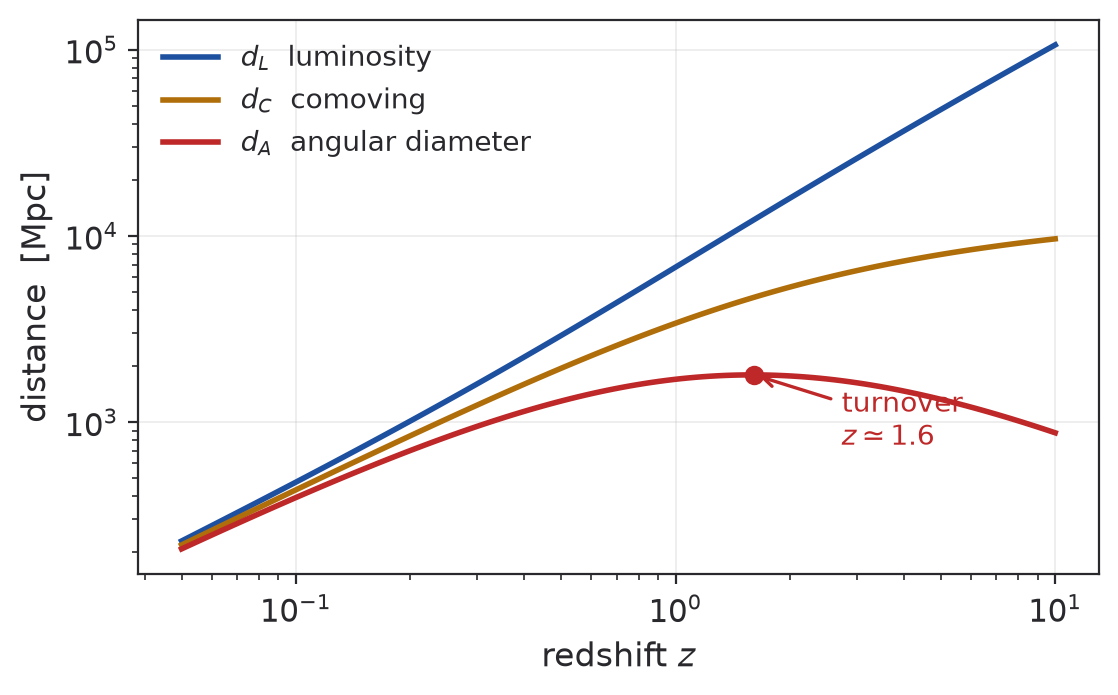
\includegraphics[width=0.72\textwidth]{fig_distances.png}
\end{center}
\vspace{-1ex}
\footnotesize The $d_A$ turnover near $z\simeq1.6$ is the usual angular-diameter
maximum. Curves computed with \Cosmic.
\end{frame}

\begin{frame}[fragile]{Tutorial --- CMB angular spectra}
\begin{lstlisting}
rec = recombination(c)
sp  = cmb_spectra(c, rec; lmax=1500, nk=20000)
D_l(sp, :TT)          # l(l+1)C_l/2pi in muK^2
\end{lstlisting}
\vspace{-1ex}
\begin{center}
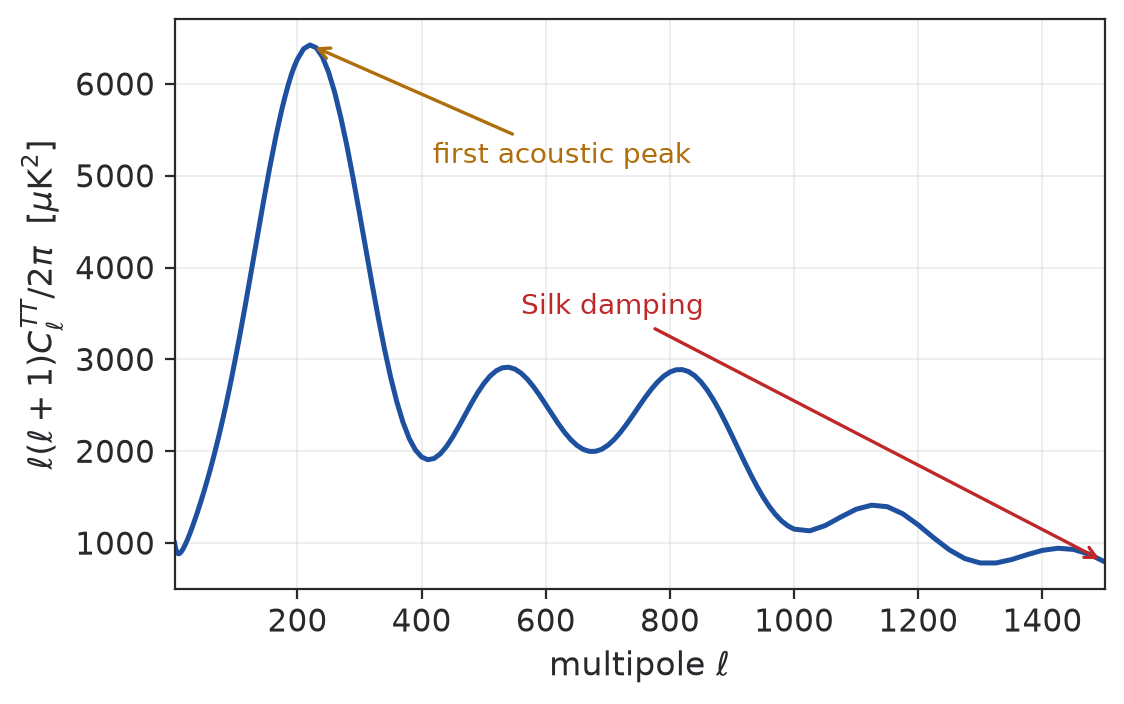
\includegraphics[width=0.72\textwidth]{fig_cls.png}
\end{center}
\vspace{-1ex}
\footnotesize Acoustic peaks and Silk damping, computed end to end from the
package's own recombination history.
\end{frame}

\begin{frame}{\Cosmic\ against CLASS}
\begin{center}
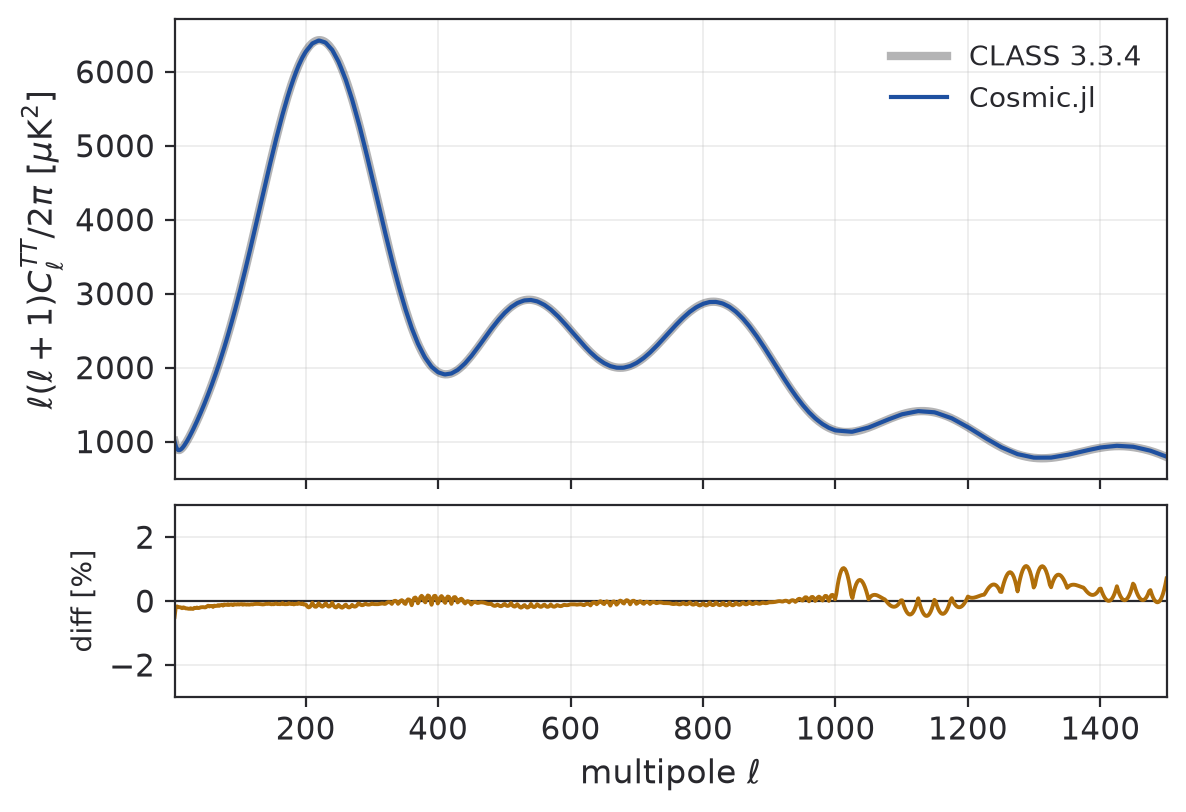
\includegraphics[width=0.70\textwidth]{fig_cls_compare.png}
\end{center}
\vspace{-1ex}
Same parameters on both sides, same $Y_p$, no reionization on either. The two
curves overlay: the residual is under \textbf{0.5\%} below $\ell\approx1000$ and
$\le1.1\%$ out to $\ell=1500$.
\begin{block}{Convergence first, physics second}
  My first attempt at this figure showed 8\% ringing near the first peak. That
  was not physics: \Cosmic\ had \emph{warned} that its $k$-grid was
  under-resolved ($\Delta k=7.9\times10^{-5}$ against a required
  $1.2\times10^{-5}$). Raising \texttt{nk} to 20000 removed it. Always converge
  both sides before reading a difference as a discrepancy.
\end{block}
\end{frame}

\begin{frame}[fragile]{Tutorial --- matter power, linear and non-linear}
\begin{lstlisting}
mp = matter_power_spectrum(c, rec; kmin=1e-3, kmax=10.0)
hf = halofit_power(mp)          # Takahashi 2012 (+Bird)
\end{lstlisting}
\vspace{-1ex}
\begin{center}
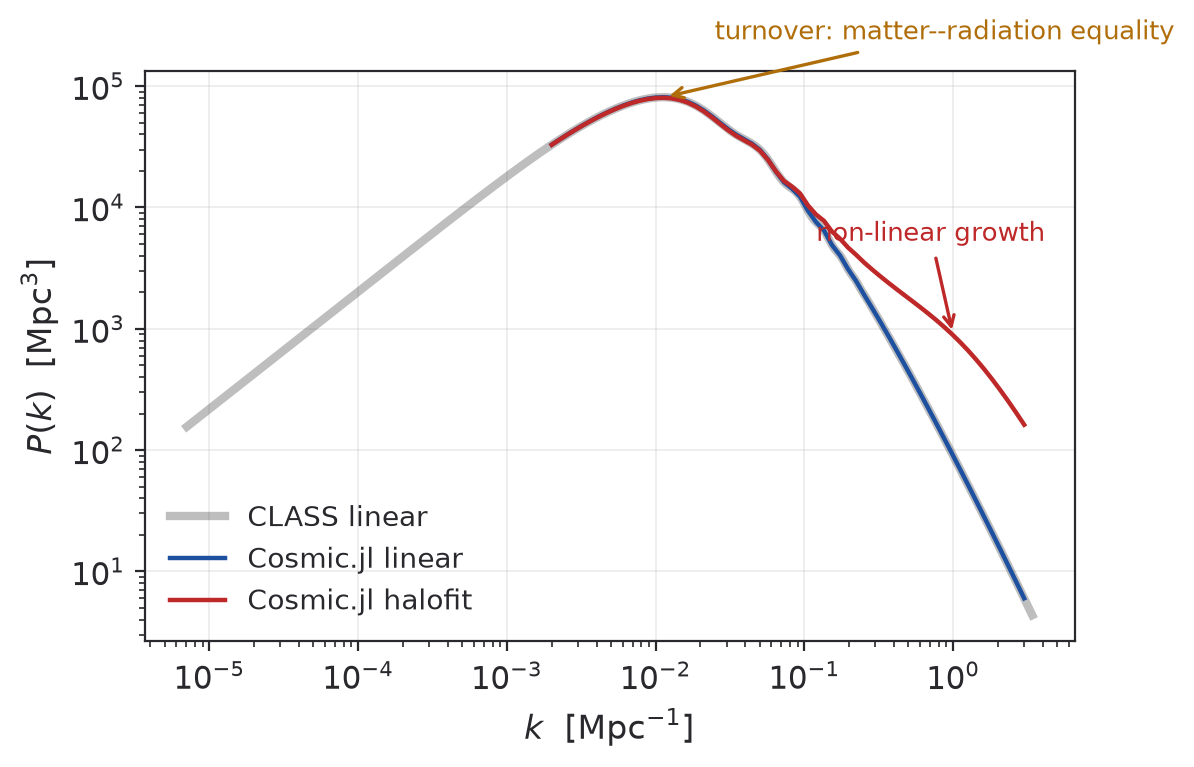
\includegraphics[width=0.72\textwidth]{fig_pk.png}
\end{center}
\vspace{-1ex}
\footnotesize Non-linear power rises above the linear spectrum for
$k\gtrsim0.1\,$Mpc$^{-1}$. HMcode-2020 and an EFT 1-loop spectrum are also
available.
\end{frame}

% =============================================================================
\section{Distinctive}

\begin{frame}{Four things that are unusual}
  \begin{block}{BBN is solved, not tabulated}
    CLASS interpolates a precomputed $Y_p(\omega_b,\Delta N)$ table; CAMB uses a
    fitting function. \Cosmic\ integrates the 12-nuclide, 63-reaction network in
    the same background, so $Y_p$ feeds recombination self-consistently.
  \end{block}
  \begin{block}{Curvature without the flat-Bessel shortcut}
    Hyperspherical Bessel functions are solved from their own recurrences at
    \emph{every} $\nu$. CLASS switches to rescaled flat Bessels above
    $\nu=4000$; here that substitution is never made.
  \end{block}
  \begin{block}{Spectral distortions from first principles}
    Exact Karzas--Latter Gaunt factor ($_2F_1$ closed form), exact
    double-Compton emissivity, and the exact Klein--Nishina $\otimes$
    Maxwell--J\"uttner Compton kernel in place of the Kompaneets approximation.
  \end{block}
  \begin{block}{Early-universe GW phenomenology}
    Scalar-induced gravitational waves and PBH abundances, including primordial
    non-Gaussianity ($f_{\rm NL}$, $g_{\rm NL}$).
  \end{block}
\end{frame}

\begin{frame}{Worked example: why ``compute, don't fit'' matters}
  The thermalization of a $\mu$-distortion needs the photon--electron
  scattering kernel. The standard choice is the \alert{Kompaneets} diffusion
  approximation.
  \vfill
  \Cosmic\ instead builds the exact isotropic Compton kernel:
  \begin{itemize}
    \item tree-level trace generated independently and checked against the
      invariant Klein--Nishina expression to $4\times10^{-11}$;
    \item folded over a relativistic Maxwell--J\"uttner electron distribution;
    \item solved by a detailed-balance finite-element weak form, which conserves
      photon number \emph{exactly} and satisfies a discrete $H$ theorem.
  \end{itemize}
  \vfill
  \begin{block}{Result}
    At matched resolution the exact kernel lands within $\sim0.1$--$0.2\%$ of
    the Kompaneets baseline: the swap is closure-neutral. The point is not that
    the answer moved --- it is that the approximation is now \emph{bounded}
    rather than assumed.
  \end{block}
\end{frame}

% =============================================================================
\section{CLASS vs CAMB vs Cosmic}

\begin{frame}{CLASS, CAMB and \Cosmic\ side by side}
  \renewcommand{\arraystretch}{1.15}
  \begin{center}\scriptsize
  \begin{tabular}{@{}llll@{}}
    \toprule
     & \textbf{CAMB} & \textbf{CLASS} & \Cosmic \\
    \midrule
    First release   & 2000 & 2011 & in development \\
    Language        & Fortran 90 & C & Julia \\
    Interface       & Python wrapper & \texttt{classy} wrapper & native \\
    Hierarchy       & TAM / line of sight & line of sight & line of sight \\
    Recombination   & RECFAST, HyRec, CosmoRec & RECFAST, HyRec & RECFAST-class, HyRec-2020 \\
    BBN             & fitting formula & interpolated table & solved network \\
    Curvature       & exact & flat approx.\ above $\nu=4000$ & exact at all $\nu$ \\
    Non-linear      & halofit, HMcode & halofit, HMcode & halofit, HMcode, EFT \\
    Distortions     & --- & fit-based & from first principles \\
    Maturity        & \textcolor{cdeep}{very high} & \textcolor{cdeep}{very high} & \alert{young} \\
    \bottomrule
  \end{tabular}
  \end{center}
  \vfill
  \footnotesize CAMB and CLASS are the references here. The honest summary is
  that \Cosmic\ reproduces them, not the other way round.
\end{frame}

\begin{frame}{How closely does it agree?}
  Cross-checks at \emph{matched settings} against live CLASS 3.3.4 and CAMB runs:
  \renewcommand{\arraystretch}{1.2}
  \begin{center}\small
  \begin{tabular}{@{}lll@{}}
    \toprule
    \textbf{Quantity} & \textbf{Reference} & \textbf{Agreement} \\
    \midrule
    Distances                 & CLASS  & $10^{-9}$ \\
    $P(k)$, $\sigma_8$        & CAMB   & $0.04\%$, $0.007\%$ \\
    $\cl^{TT}$ (unlensed)     & CLASS  & $\sim0.4\%$ \\
    Lensed $TT$ / $EE$        & CLASS  & $0.3\%$ / $0.4\%$ \\
    $\cl^{\phi\phi}$ ($\ell\le1000$) & CLASS & $\le0.9\%$ \\
    halofit ratio $P_{\rm nl}/P_{\rm lin}$ & CLASS & $0.25\%$ \\
    EFT 1-loop $P_{22}+P_{13}$ & FAST-PT & $<0.5\%$ \\
    $Y_p$                     & CLASS (PRIMAT) & $<0.1\%$ \\
    $Y_p$, D/H, $^7$Li        & PRyMordial & $-0.004\%$, $+0.03\%$, $-1.1\%$ \\
    $\mu$, $y$                & CLASS  & $0.02\%$ \\
    Open / closed $\cl^{TT}$  & CLASS / CAMB & $\le0.6\%$ / $\le0.4\%$ \\
    \bottomrule
  \end{tabular}
  \end{center}
\end{frame}

\begin{frame}{A comparison trap worth knowing}
  Low-$\ell$ $\cl^{TT}$ receives a large contribution from $k\gg\ell/\eta_0$ ---
  at $\ell=20$ the tail supplies $\sim35\%$ of the power.
  \vfill
  CLASS and CAMB tie their $k_{\max}$ to \texttt{l\_max}. So an isolated run with
  \texttt{l\_max\_scalars=30} is \alert{badly under-converged}:
  \[
    \cl^{TT}(\ell=20):\quad 721\ \text{(default)}\ \longrightarrow\ 993\ \text{(converged)}
  \]
  while a full $\ell_{\max}\simeq2500$ run is fine automatically.
  \vfill
  \begin{block}{Rule}
    Never compare low-$\ell$-only runs without matching \emph{absolute}
    $k_{\max}$ on both sides. More than one ``bug'' in this project turned out
    to be a reference run that was not converged.
  \end{block}
\end{frame}

% =============================================================================
\section{Status}

\begin{frame}{What is not there yet --- and what is approximate}
  \begin{block}{Missing}
    Vector modes; number-count and shear spectra; late-time $y$-distortion;
    scalar-field and interacting dark-energy perturbations; a second-order
    (bispectrum) solver.
  \end{block}
  \begin{block}{Known approximation, stated plainly}
    Non-scalar modes use the \emph{optimal} Boltzmann hierarchy, which
    re-expands them on scalar normal modes. Pitrou, Pereira \& Lesgourgues
    (PRD~102, 023511) show the separability this relies on \alert{fails at
    $K\neq0$}: the error is negligible for scalars but reaches
    $\sim50\,|\Omega_K|\%$ on \emph{tensor polarization}. So curved tensor
    $EE/BB$ is currently an inherited approximation, not an exact result.
  \end{block}
  \vfill
  \footnotesize Being explicit about this is the point. A code that only lists
  its successes is harder to trust than one that names its error terms.
\end{frame}

\begin{frame}{Roadmap}
  \begin{enumerate}
    \item Vector modes, and the scalar\,+\,vector\,+\,tensor sum.
    \item Dark-matter variants: warm, decaying, annihilating, interacting.
    \item Dark-energy perturbations and quintessence.
    \item Modified gravity in the stable EFT-of-dark-energy basis.
    \item Number counts and galaxy/shear $\cl$.
    \item Second order: scalar-induced GWs first, then the intrinsic bispectrum.
    \item Neutrino quantum kinetics ($N_{\rm eff}:3.0428\to3.044$).
    \item Differentiability end to end, then gradient-based inference.
  \end{enumerate}
\end{frame}

\begin{frame}{Summary}
  \begin{itemize}
    \item \Cosmic\ is a pure-Julia cosmology and Einstein--Boltzmann engine:
      background $\to$ BBN $\to$ recombination $\to$ perturbations $\to$
      CMB/LSS, coupled through one composition.
    \item It reproduces CLASS and CAMB at the few-$10^{-3}$ level across
      distances, $\cl$, $P(k)$, BBN abundances and spectral distortions.
    \item Its distinctive choices are a generic species design, exact curved
      geometry, a solved BBN network, and first-principles distortion physics.
    \item It is young. CAMB and CLASS remain the references, and the open
      approximations are documented rather than hidden.
  \end{itemize}
  \vfill
  \begin{center}
    \textcolor{cdeep}{\texttt{github.com/aburousan/Cosmic.jl}}\\[0.5ex]
    \small Kazi Abu Rousan
  \end{center}
\end{frame}

\end{document}
